\chapter{Example}
\label{chap:examples}

In this chapter we will introduce an example scenario of a process and how the resulting code of the transformation looks like.

\section{The Model}
The example is based on a scenario taken from an actual topic: \textit{electromobility}. The scenario includes a choreography between a MobileApplication, that will be used by a user to reserve a taxi and a number of ETaxi-applications installed in electronic taxis. Figure \ref{fig:usecase} shows the use case model of the \textbf{requestTaxi} process. 
\begin{figure}[h]
	\centering
		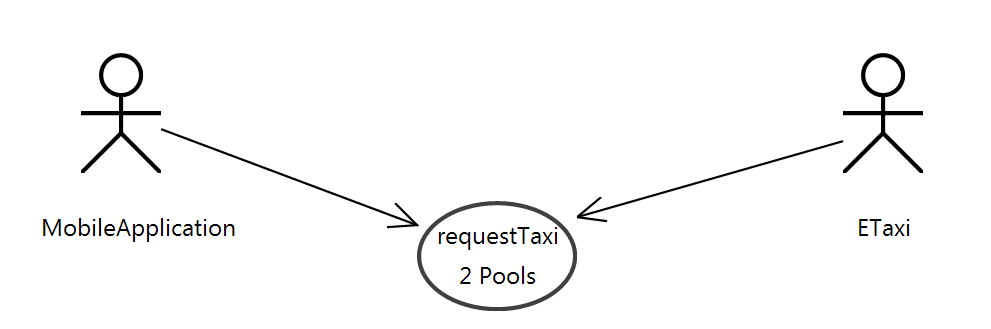
\includegraphics[width=0.8\textwidth]{images/example/usecase.png}
	\label{fig:usecase}
	\caption{Use Case Model}
\end{figure}

In figure \ref{fig:payloads} we can see some data types included in the process which represent the information exchanged in the communication between both pools (the payload of the implementing MessageChannel). The transformation will assume that the classes exist and they will be imported by the generated Agent Bean. Further, because payloads will be wrapped in a JiacMessage, they have to implement the IFact interface.
\begin{figure}[h]
	\centering
		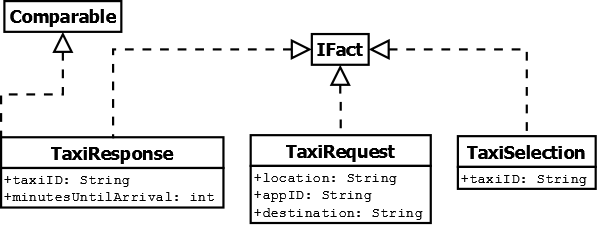
\includegraphics[width=0.8\textwidth]{images/example/payloads.png}
	\label{fig:payloads}
	\caption{Payload data types included in the process diagram}
\end{figure}

\newpage
\subsection{The scenario}
Before we start with the transformation, we will describe the scenario that lies behind the process model shown in figure \ref{fig:example} from the perspective of each pool. 

\textbf{Mobile Application}\\
The process starts with a user requesting a taxi by invoking the service provided by the mobile application. The service will then make a request to all ETaxis by sending information about the user's location, application ID and the destination. Within 30 seconds after sending the request, the mobile application will collect responses from all available ETaxis. Each of these responses contains information about the taxi ID and the estimated time needed by this taxi to arrive at the user's current location. If multiple responses are received, the mobile application will record the best response according to the minimum estimated time. After 30 seconds the application will check whether a response was received. If yes, it will send a notification to all taxis informing which taxi is selected. Then the process will end and the selected taxi's ID will be sent to the user. If no respons is received, it will notify the user that no taxi is currently available. 


\textbf{ETaxi}\\
From the ETaxi perspective, the process starts when a request from a mobile application is received. It will then evaluate the request and decide whether or not the request is interesting e.g according to the distance between the taxi's location and the user's location. If the request is interesting, the ETaxi will then send a response back to the requesting MobileApplication. After that it will wait for a notification from the MobileApplication and check the included taxiID. If the taxiID belongs to the ETaxi, the driver will be informed and the system will navigate to the user's location.


\begin{sidewaysfigure}
	\centering
		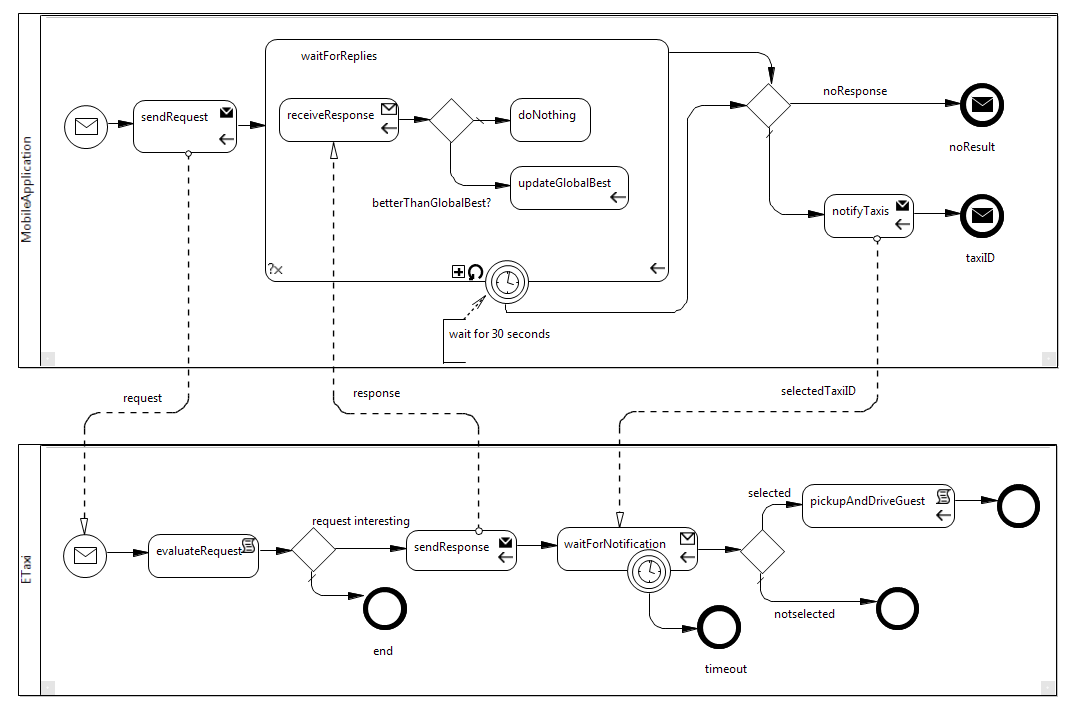
\includegraphics[width = 0.9\textwidth]{images/example/requestTaxi.png}
	\label{fig:example}
	\caption{Business Process Diagram - requestTaxi}
\end{sidewaysfigure}


\subsection{Problem With MessageChannel}
As mentioned in the open issues of the mapping, with the MessageChannel implementation, a message will be broadcasted to all subscribers of a communication group. This is a problem for our scenario since the response from the ETaxis should be sent only to the requesting MobileApplication. In order to keep the scenario as it is, we decided to make a workaround for this problem and create a channel (communication group) where the application ID (appID) is included in the address. This way each mobile application will have its own channel. 

\newpage
At the moment, the implemented element mapping will map the given channel into a String literal (the expression will be wrapped with two quotation marks \verb|"[expression]"|). Obviously we need to avoid the wrapping of the appID variable as a String literal. Therefore we constructed the channel expression as \verb|TaxiResponse-To"+appID+"|. This way the mapped expression will be \verb|"TaxiResponseTo"+appID+""|. Perhaps it would be better if we change the implementation in the future and skip the wrapping of the given expression. Instead we can simply assume that the given expression is a valid Java String literal or a String variable e.g \verb|"TaxiRequest"| or \verb|requestChannel|(requestChannel must be a String variable contained in the Agent Bean).

\section{The Generated Agent Beans}
In this section we will present the Agent Beans generated from the above model. To save space and improve the readability, the generated code will be reduced as follows:
\begin{itemize}
	\item Imports are deleted
	\item Javadoc elements used for JMerge are deleted
	\item The inner class TimeoutEventHandler which we already presented in section \ref{sec:handler} is deleted
	\item Some empty lines are deleted
\end{itemize}
Beside the mentioned reduction, no other changes were made to the generated code. All codes and comments are generated directly from the model.

\textbf{1. MobileApplication\_requestTaxi}\\

\begin{lstlisting}[language=java, caption= Generated Agent Bean - MobileApplication\_requestTaxi]
package mobileapplication;
[imports]
public class MobileApplication_requestTaxi extends AbstractMethodExposingBean{
	public final static String ACTION_REQUESTTAXI = "mobileapplication.MobileApplication_requestTaxi#requestTaxi"; 
	
	TaxiResponse globalBest;
	boolean noResponse;
	String appID;
	String location;
	String destination;
	
	@Expose(name = ACTION_REQUESTTAXI, scope = ActionScope.GLOBAL)
	public String requestTaxi(String currentLocation, String currentDestination) {
		location= currentLocation;
		destination= currentDestination;
		sendRequest();
		Thread waitForReplies = new Thread(new Runnable(){
			public void run(){
				WaitForRepliesSubProcess waitForReplies = new WaitForRepliesSubProcess();
				waitForReplies.run();
			}
		});
		TimeoutEventHandler wait30Seconds_TimeoutHandler = new TimeoutEventHandler(30000,waitForReplies);
		waitForReplies.start();
		wait30Seconds_TimeoutHandler.start();
		try {
			waitForReplies.join();
			wait30Seconds_TimeoutHandler.stop();
		} catch(InterruptedException e) {
		}
		
		if(noResponse){
			String taxiID;
			taxiID= "none available";
			return taxiID;
		} else {
			notifyTaxis();
			String taxiID;
			taxiID= globalBest.getTaxiID();
			return taxiID;
		}
	}

	private void sendRequest() {
		TaxiRequest request;
		request= new TaxiRequest(location,appID,destination);
		Action sendAction = retrieveAction(ICommunicationBean.ACTION_SEND);
		IGroupAddress groupAddress = CommunicationAddressFactory.createGroupAddress("TaxiRequest");
		JiacMessage jiacMessage = new JiacMessage(request);
		invoke(sendAction, new Serializable[]{jiacMessage, groupAddress});
	}

	private void notifyTaxis() {
		SelectedTaxi selectedTaxi;
		selectedTaxi= new SelectedTaxi(globalBest.getTaxiID());
		Action sendAction = retrieveAction(ICommunicationBean.ACTION_SEND);
		IGroupAddress groupAddress = CommunicationAddressFactory.createGroupAddress("notification");
		JiacMessage jiacMessage = new JiacMessage(selectedTaxi);
		invoke(sendAction, new Serializable[]{jiacMessage, groupAddress});
	}

	class WaitForRepliesSubProcess{
		
		TaxiResponse currentResponse;
		
		public void run() {
			noResponse= true;
			while(true) {
				receiveResponse();
				if(currentResponse.compareTo(globalBest)>0){
					updateGlobalBest();
				} else {
					doNothing();
				}
			}
		}
	 
		private void receiveResponse() {
			Action joinAction = retrieveAction(ICommunicationBean.ACTION_JOIN_GROUP);
			Action leaveAction = retrieveAction(ICommunicationBean.ACTION_LEAVE_GROUP);
			IGroupAddress groupAddress = CommunicationAddressFactory.createGroupAddress("TaxiResponseTo"+appID+"");
			invoke(joinAction,new Serializable[]{groupAddress});
			TaxiResponse response = null;
			while(response==null) {
				Set<IFact> all = memory.readAll();
				for(IFact fact : all){
					if(fact instanceof JiacMessage) {
						JiacMessage jiacMessage = (JiacMessage)fact;
						if(jiacMessage.getPayload() instanceof TaxiResponse && jiacMessage.getHeader(IJiacMessage.Header.SEND_TO).equals("TaxiResponseTo"+appID+"")) {
							memory.remove(jiacMessage);
							response = (TaxiResponse) jiacMessage.getPayload();
							break;
						}
					}
				}
				try{
					Thread.sleep(100);
				} catch(InterruptedException e) { }
			}
			invoke(leaveAction, new Serializable[]{groupAddress});
			noResponse= false;
			currentResponse= response;
		}
	 
		private void doNothing() {
		}
	 
		private void updateGlobalBest() {
			globalBest= currentResponse;
		} 
	}
}
\end{lstlisting}

In the MobileApplication\_requestTaxi Bean, almost every logic is generated from the model. The workflow method requestTaxi is exposed as an action. All methods are filled with needed operations e.g. the decision whether the currentResponse is better than the globalBest is made by using the compareTo method of the TaxiResponse class. There is only one small yet fatal aspect missing in the generated code. You might notice that while other variables are initialized somewhere in the assignment of a method, the initialization of the appID variable can't be found in the generated code. To ensure that each instance of the MobileApplication\_requestTaxi has a unique ID, the initialization cannot be included in the model. We have to e.g. add a constructor and implement the initialization of the appID in it to make the code works completely. This problem also exists in the generated ETaxi\_requestTaxi code.

\textbf{2. ETaxi\_requestTaxi}\\

\begin{lstlisting}[language=java, caption= Generated Agent Bean - ETaxi\_requestTaxi]
package etaxi;
[imports]
public class ETaxi_requestTaxi extends AbstractMethodExposingBean{
	public final static String ACTION_REQUESTTAXI = "etaxi.ETaxi_requestTaxi#requestTaxi"; 

	boolean requestInteresting;
	String taxiID;
	String globalLocation;
	int estimatedTime;
	String appID;
	TaxiRequest currentRequest;
	SelectedTaxi selection;
	boolean available;

	@Expose(name = ACTION_REQUESTTAXI, scope = ActionScope.GLOBAL)
	public void requestTaxi(TaxiRequest request) {
		currentRequest= request;
		evaluateRequest();
		if(requestInteresting){
			sendResponse();
			Thread waitForNotification = new Thread(new Runnable(){
				public void run(){
					waitForNotification();
				}
			});
			TimeoutEventHandler _x5RCUAGWEeGC8PuSIWxlmQ_TimeoutHandler = new TimeoutEventHandler(60000,waitForNotification);
			waitForNotification.start();
			_x5RCUAGWEeGC8PuSIWxlmQ_TimeoutHandler.start();
			try {
				waitForNotification.join();
				_x5RCUAGWEeGC8PuSIWxlmQ_TimeoutHandler.stop();
			} catch(InterruptedException e) {
			}
			if(!_x5RCUAGWEeGC8PuSIWxlmQ_TimeoutHandler.hasBeenTriggered()){
				if(selection.getTaxiID().equals(taxiID)){
					pickupAndDriveGuest();
				} else {
				}
			}
		} else {
		}
	}

	public void doStart() {
		Action joinAction = retrieveAction(ICommunicationBean.ACTION_JOIN_GROUP);
		IGroupAddress groupAddress = CommunicationAddressFactory.createGroupAddress("TaxiRequest");
		invoke(joinAction,new Serializable[]{groupAddress});
		SpaceObserver<IFact> _B8QyYAF3EeGC8PuSIWxlmQ_observer = new SpaceObserver<IFact>(){
			public void notify(SpaceEvent<? extends IFact> event) { 
				if(event instanceof WriteCallEvent){ 
					Object obj  = ((WriteCallEvent) event).getObject();
					if (obj instanceof IJiacMessage){
						IJiacMessage message = (IJiacMessage)obj;
						IFact payload = message.getPayload();
						if(payload!=null && payload instanceof TaxiRequest&& message.getHeader(IJiacMessage.Header.SEND_TO).equalsIgnoreCase("TaxiRequest")){
							memory.remove(message);
							requestTaxi((TaxiRequest)payload);
						}
					}
				}
			}
		};
		memory.attach(_B8QyYAF3EeGC8PuSIWxlmQ_observer);
	}

	private void evaluateRequest() {
		//script activity
		//TODO implement code 
		requestInteresting = true; //every request is interesting
	}

	private void sendResponse() {
		TaxiResponse response;
		response= new TaxiResponse(taxiID, estimatedTime);
		Action sendAction = retrieveAction(ICommunicationBean.ACTION_SEND);
		IGroupAddress groupAddress = CommunicationAddressFactory.createGroupAddress("TaxiResponseTo"+appID+"");
		JiacMessage jiacMessage = new JiacMessage(response);
		invoke(sendAction, new Serializable[]{jiacMessage, groupAddress});
	}

	private void waitForNotification() {
		Action joinAction = retrieveAction(ICommunicationBean.ACTION_JOIN_GROUP);
		Action leaveAction = retrieveAction(ICommunicationBean.ACTION_LEAVE_GROUP);
		IGroupAddress groupAddress = CommunicationAddressFactory.createGroupAddress("notification");
		invoke(joinAction,new Serializable[]{groupAddress});
		SelectedTaxi selectedTaxi = null;
		while(selectedTaxi==null) {
			Set<IFact> all = memory.readAll();
			for(IFact fact : all){
				if(fact instanceof JiacMessage) {
					JiacMessage jiacMessage = (JiacMessage)fact;
					if(jiacMessage.getPayload() instanceof SelectedTaxi && jiacMessage.getHeader(IJiacMessage.Header.SEND_TO).equals("notification")) {
						memory.remove(jiacMessage);
						selectedTaxi = (SelectedTaxi) jiacMessage.getPayload();
						break;
					}
				}
			}
			try{
				Thread.sleep(100);
			} catch(InterruptedException e) { }
		}
		invoke(leaveAction, new Serializable[]{groupAddress});
		selection= selectedTaxi;
	}

	private void pickupAndDriveGuest() {
		available= false;
		// TODO add code to navigate to guest's location
		available= true;
	}
	
}
\end{lstlisting}

Similar to the MobileApplication\_requestTaxi Bean, the initialization of the taxiID is also missing in the generated code. Moreover, unlike the MobileApplication\_request-Taxi Agent Bean, we did not include all the logic in the model (e.g. for evaluating whether a request is interesting). By this we showed that the quantity of the generated code might vary depending on how we design the model.


In this chapter we have presented an example of the transformation in which some problems regarding the current mapping and transformation are shown. We have also shown how agents can be designed and created easily by modeling a business process. 
